\documentclass[tikz]{standalone}

\usepackage{tikz}
\usetikzlibrary{trees}
\usetikzlibrary{shapes}
\usetikzlibrary{positioning}
\usetikzlibrary{arrows.meta}

\tikzset{
    pointer/.style = {thick,draw=black,triangle 45-*,shorten >=-3pt},
    cell/.style = {rectangle, thick, draw=black,minimum width = 1cm, minimum height =1.0cm,fill=yellow!20},
    mynode/.style = {circle, thick, draw=black, align=center,fill=yellow!40,font=\ttfamily\bfseries\Large},
    mynoder/.style = {circle, thick, draw=black, align=center,fill=red!30,font=\ttfamily\bfseries\Large},
    mynodeb/.style = {circle, thick, draw=black, align=center,fill=blue!30,font=\ttfamily\bfseries\Large},
    edgen/.style = {-latex,ultra thick},
    edger/.style = {-latex,ultra thick,red},
    edgeb/.style = {-latex,ultra thick,blue},
    edgeg/.style = {-latex,ultra thick,gray},
    edgegd/.style = {-latex,ultra thick,brown,dashed}, % back
    edgevd/.style = {-latex,ultra thick,violet,dotted}, % forward
    edgexd/.style = {-latex,ultra thick,blue,densely dotted}, % traversal
    every picture/.style={/utils/exec={\ttfamily\bfseries}},
    every picture/.style={font issue=\ttfamily\bfseries},
    font issue/.style={execute at begin picture={#1\selectfont}
  }
}

\begin{document}

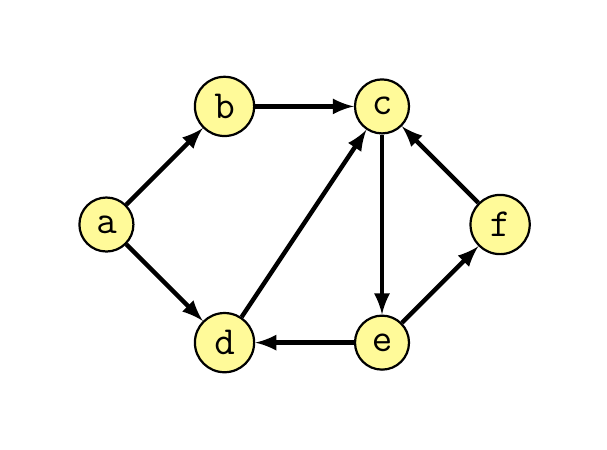
\begin{tikzpicture}[scale=1.00,transform shape]
%
\node[mynode] at (0.5,0) (a) {a};
\node[mynode] at (2,1.5) (b) {b};
\node[mynode] at (4,1.5) (c) {c};
\node[mynode] at (2,-1.5) (d) {d};
\node[mynode] at (4,-1.5) (e) {e};
\node[mynode] at (5.5,0) (f) {f};
%
\draw[edgen] (a) edge node {} (b);
\draw[edgen] (a) edge node {} (d);
\draw[edgen] (b) edge node {} (c);
\draw[edgen] (c) edge node {} (e);
\draw[edgen] (e) edge node {} (d);
\draw[edgen] (f) edge node {} (c);
\draw[edgen] (e) edge node {} (f);
\draw[edgen] (d) edge node {} (c);

\path[use as bounding box] (-0.5,-2.5) rectangle (6.5, 2.5);

\end{tikzpicture}

\newpage

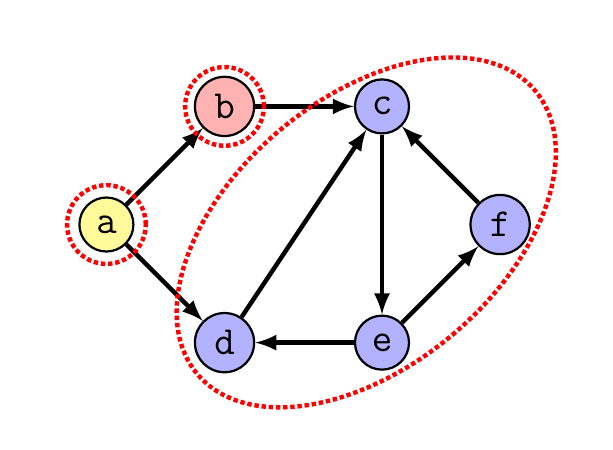
\begin{tikzpicture}[scale=1.00,transform shape]
%
\node[mynode] at (0.5,0) (a) {a};
\node[mynoder] at (2,1.5) (b) {b};
\node[mynodeb] at (4,1.5) (c) {c};
\node[mynodeb] at (2,-1.5) (d) {d};
\node[mynodeb] at (4,-1.5) (e) {e};
\node[mynodeb] at (5.5,0) (f) {f};
%
\draw[edgen] (a) edge node {} (b);
\draw[edgen] (a) edge node {} (d);
\draw[edgen] (b) edge node {} (c);
\draw[edgen] (c) edge node {} (e);
\draw[edgen] (e) edge node {} (d);
\draw[edgen] (f) edge node {} (c);
\draw[edgen] (e) edge node {} (f);
\draw[edgen] (d) edge node {} (c);

\draw[ultra thick,red,densely dotted] (0.5,0) circle (0.5cm);
\draw[ultra thick,red,densely dotted] (2,1.5) circle (0.5cm);
\draw[ultra thick,red,densely dotted,rotate around={-50:(3.8,-0.1)}] (3.8,-0.1) ellipse (1.7cm and 2.8cm);

\path[use as bounding box] (-0.5,-2.5) rectangle (6.5, 2.5);

%[,red]
\end{tikzpicture}

\newpage

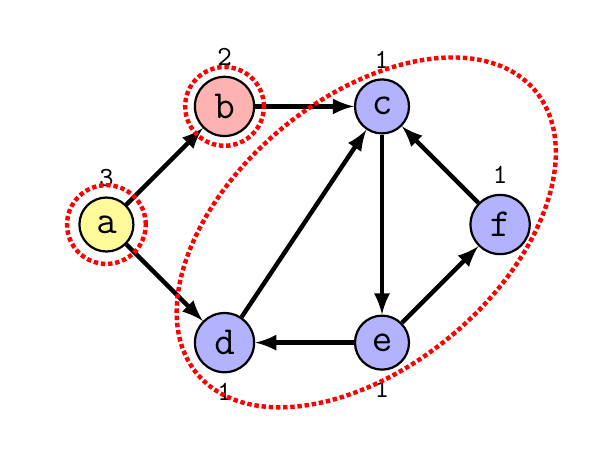
\begin{tikzpicture}[scale=1.00,transform shape]
%
\node[mynode, label={3}] at (0.5,0) (a) {a};
\node[mynoder, label={2}] at (2,1.5) (b) {b};
\node[mynodeb, label={1}] at (4,1.5) (c) {c};
\node[mynodeb, label={below:1}] at (2,-1.5) (d) {d};
\node[mynodeb, label={below:1}] at (4,-1.5) (e) {e};
\node[mynodeb, label={1}] at (5.5,0) (f) {f};
%
\draw[edgen] (a) edge node {} (b);
\draw[edgen] (a) edge node {} (d);
\draw[edgen] (b) edge node {} (c);
\draw[edgen] (c) edge node {} (e);
\draw[edgen] (e) edge node {} (d);
\draw[edgen] (f) edge node {} (c);
\draw[edgen] (e) edge node {} (f);
\draw[edgen] (d) edge node {} (c);

\draw[ultra thick,red,densely dotted] (0.5,0) circle (0.5cm);
\draw[ultra thick,red,densely dotted] (2,1.5) circle (0.5cm);
\draw[ultra thick,red,densely dotted,rotate around={-50:(3.8,-0.1)}] (3.8,-0.1) ellipse (1.7cm and 2.8cm);

\path[use as bounding box] (-0.5,-2.5) rectangle (6.5, 2.5);

\end{tikzpicture}

\newpage

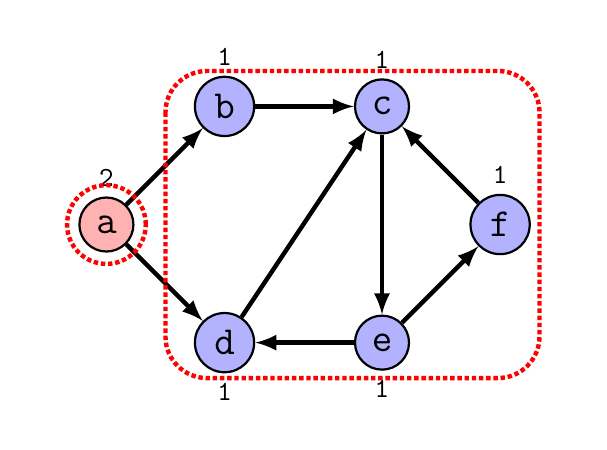
\begin{tikzpicture}[scale=1.00,transform shape]
%
\node[mynoder, label={2}] at (0.5,0) (a) {a};
\node[mynodeb, label={1}] at (2,1.5) (b) {b};
\node[mynodeb, label={1}] at (4,1.5) (c) {c};
\node[mynodeb, label={below:1}] at (2,-1.5) (d) {d};
\node[mynodeb, label={below:1}] at (4,-1.5) (e) {e};
\node[mynodeb, label={1}] at (5.5,0) (f) {f};
%
\draw[edgen] (a) edge node {} (b);
\draw[edgen] (a) edge node {} (d);
\draw[edgen] (b) edge node {} (c);
\draw[edgen] (c) edge node {} (e);
\draw[edgen] (e) edge node {} (d);
\draw[edgen] (f) edge node {} (c);
\draw[edgen] (e) edge node {} (f);
\draw[edgen] (d) edge node {} (c);

\draw[ultra thick,red,densely dotted] (0.5,0) circle (0.5cm);
\draw[ultra thick,red,densely dotted,rounded corners=15pt] (1.25,1.95) rectangle (6,-1.95);

\path[use as bounding box] (-0.5,-2.5) rectangle (6.5, 2.5);

\end{tikzpicture}

\newpage

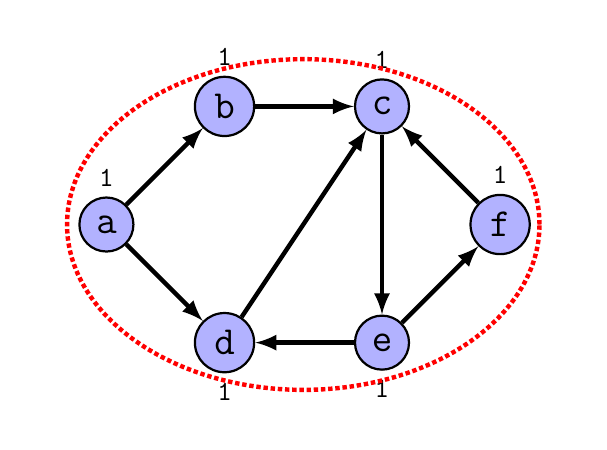
\begin{tikzpicture}[scale=1.00,transform shape]
%
\node[mynodeb, label={1}] at (0.5,0) (a) {a};
\node[mynodeb, label={1}] at (2,1.5) (b) {b};
\node[mynodeb, label={1}] at (4,1.5) (c) {c};
\node[mynodeb, label={below:1}] at (2,-1.5) (d) {d};
\node[mynodeb, label={below:1}] at (4,-1.5) (e) {e};
\node[mynodeb, label={1}] at (5.5,0) (f) {f};
%
\draw[edgen] (a) edge node {} (b);
\draw[edgen] (a) edge node {} (d);
\draw[edgen] (b) edge node {} (c);
\draw[edgen] (c) edge node {} (e);
\draw[edgen] (e) edge node {} (d);
\draw[edgen] (f) edge node {} (c);
\draw[edgen] (e) edge node {} (f);
\draw[edgen] (d) edge node {} (c);

\draw[ultra thick,red,densely dotted] (3,0) ellipse (3cm and 2.1cm);

\path[use as bounding box] (-0.5,-2.5) rectangle (6.5, 2.5);

\end{tikzpicture}


\end{document}